\documentclass[12pt,a4paper]{report}

% ============================================================
%  SHARED METADATA
% ============================================================
% ============================================================
%  meta.tex — shared metadata for the report (main.tex) and slides (slides/slides.tex)
%  Edit here only; both documents \input this file.
% ============================================================
\newcommand{\metaUniversity}{Đại học Bách khoa Hà Nội}
\newcommand{\metaSchool}{Trường Công nghệ Thông tin và Truyền thông}
\newcommand{\metaCourse}{Seminar 1}
\newcommand{\metaTopicCode}{A1}
\newcommand{\metaTitle}{Dùng AI phát hiện mơ hồ, thiếu sót, mâu thuẫn trong tài liệu đặc tả yêu cầu}
\newcommand{\metaShortTitle}{A1 -- AI phát hiện lỗi đặc tả yêu cầu}
\newcommand{\metaLecturer}{TS. Nguyễn Thanh Hùng}
\newcommand{\metaLecturerUnit}{Khoa Khoa học Máy tính}
\newcommand{\metaGroup}{Nhóm 4}
\newcommand{\metaSemester}{Học kỳ 20252 --- Năm học 2025--2026}
\newcommand{\metaDate}{\today}

% Members table body (ID & Name & Role)
\newcommand{\metaMembers}{%
  20251175M & Nguyễn Tùng Dương & Nhóm trưởng \\
  20251177M & Trần Xuân Nam     & Thành viên \\
  20252636M & Phạm Gia Khánh    & Thành viên \\
}
% Short author line for slide footer / title
\newcommand{\metaAuthorsShort}{Nguyễn Tùng Dương, Trần Xuân Nam, Phạm Gia Khánh}

% Generated by script/export_numbers.py -- do not edit by hand.
\newcommand{\numAIRevBorder}{4}
\newcommand{\numAIRevExpN}{5}
\newcommand{\numAIRevExpReal}{4}
\newcommand{\numAIRevN}{25}
\newcommand{\numAIRevNonReq}{4}
\newcommand{\numAIRevNot}{12}
\newcommand{\numAIRevOverLiteral}{8}
\newcommand{\numAIRevReal}{9}
\newcommand{\numAIRevRealHi}{52}
\newcommand{\numAIRevRealLo}{36}
\newcommand{\numAgyMTokens}{1{,}85}
\newcommand{\numAgyMinutes}{123}
\newcommand{\numDurTfour}{206}
\newcommand{\numDurTone}{91}
\newcommand{\numDurTthree}{211}
\newcommand{\numDurTtwo}{110}
\newcommand{\numEffortTfour}{2{,}5}
\newcommand{\numEffortTone}{4{,}0}
\newcommand{\numEffortTthree}{3{,}5}
\newcommand{\numEffortTtwo}{2{,}7}
\newcommand{\numEffortTzero}{2{,}5}
\newcommand{\numFAllTfour}{67{,}0}
\newcommand{\numFAllTone}{50{,}8}
\newcommand{\numFAllTthree}{55{,}3}
\newcommand{\numFAllTtwo}{63{,}8}
\newcommand{\numFAllTzero}{48{,}7}
\newcommand{\numFAmbTfour}{62}
\newcommand{\numFAmbTone}{37}
\newcommand{\numFAmbTthree}{42}
\newcommand{\numFAmbTtwo}{59}
\newcommand{\numFAmbTzero}{67}
\newcommand{\numFConTfour}{76}
\newcommand{\numFConTone}{79}
\newcommand{\numFConTthree}{69}
\newcommand{\numFConTtwo}{89}
\newcommand{\numFConTzero}{62}
\newcommand{\numFFlagAll}{27{,}9}
\newcommand{\numFIncTfour}{46}
\newcommand{\numFIncTone}{37}
\newcommand{\numFIncTthree}{39}
\newcommand{\numFIncTtwo}{41}
\newcommand{\numFIncTzero}{23}
\newcommand{\numFLenTfour}{69{,}7}
\newcommand{\numFLenTone}{64{,}2}
\newcommand{\numFLenTthree}{65{,}2}
\newcommand{\numFLenTtwo}{69{,}4}
\newcommand{\numFLenTzero}{52{,}0}
\newcommand{\numFSeedTfour}{100{,}0}
\newcommand{\numFSeedTone}{96{,}1}
\newcommand{\numFSeedTthree}{100{,}0}
\newcommand{\numFSeedTtwo}{97{,}8}
\newcommand{\numFSeedTzero}{65{,}3}
\newcommand{\numFTfour}{55{,}6}
\newcommand{\numFTone}{40{,}3}
\newcommand{\numFTthree}{43{,}9}
\newcommand{\numFTtwo}{52{,}8}
\newcommand{\numFTzero}{41{,}1}
\newcommand{\numFhiTfour}{63{,}2}
\newcommand{\numFhiTone}{47{,}0}
\newcommand{\numFhiTthree}{50{,}9}
\newcommand{\numFhiTtwo}{60{,}1}
\newcommand{\numFhiTzero}{51{,}9}
\newcommand{\numFleissTfour}{0{,}89}
\newcommand{\numFleissTone}{0{,}89}
\newcommand{\numFleissTthree}{0{,}77}
\newcommand{\numFleissTtwo}{0{,}83}
\newcommand{\numFloTfour}{47{,}0}
\newcommand{\numFloTone}{33{,}2}
\newcommand{\numFloTthree}{36{,}4}
\newcommand{\numFloTtwo}{45{,}0}
\newcommand{\numFloTzero}{29{,}7}
\newcommand{\numFoundTfour}{122}
\newcommand{\numFoundTone}{206}
\newcommand{\numFoundTthree}{185}
\newcommand{\numFoundTtwo}{135}
\newcommand{\numFsdTfour}{1{,}0}
\newcommand{\numFsdTone}{1{,}3}
\newcommand{\numFsdTthree}{4{,}1}
\newcommand{\numFsdTtwo}{2{,}2}
\newcommand{\numFsdTzero}{0{,}0}
\newcommand{\numGTPure}{52}
\newcommand{\numHCSlideA}{\textbf{[Đang chờ kết quả kiểm tra bởi người]}}
\newcommand{\numHCSlideB}{\textbf{[Đang chờ kết quả kiểm tra bởi người]}}
\newcommand{\numHCSlideC}{\textbf{[Đang chờ kết quả kiểm tra bởi người]}}
\newcommand{\numHumanCheckDone}{0}
\newcommand{\numJacTfour}{0{,}87}
\newcommand{\numJacTone}{0{,}93}
\newcommand{\numJacTthree}{0{,}82}
\newcommand{\numJacTtwo}{0{,}83}
\newcommand{\numLeakMaxShift}{3{,}9}
\newcommand{\numMissTfour}{7{,}1}
\newcommand{\numMissTone}{0{,}0}
\newcommand{\numMissTthree}{0{,}6}
\newcommand{\numMissTtwo}{5{,}1}
\newcommand{\numMissTzero}{57{,}7}
\newcommand{\numModelDFPlain}{3{,}7}
\newcommand{\numModelDFSkill}{2{,}8}
\newcommand{\numModelHiPlain}{5{,}3}
\newcommand{\numModelHiSkill}{5{,}3}
\newcommand{\numModelLoPlain}{2{,}2}
\newcommand{\numModelLoSkill}{0{,}1}
\newcommand{\numPFlagAll}{16{,}2}
\newcommand{\numPTfour}{39{,}7}
\newcommand{\numPTone}{25{,}2}
\newcommand{\numPTthree}{28{,}3}
\newcommand{\numPTtwo}{36{,}6}
\newcommand{\numPTzero}{40{,}0}
\newcommand{\numRAmbTfour}{92}
\newcommand{\numRAmbTone}{100}
\newcommand{\numRAmbTthree}{100}
\newcommand{\numRAmbTtwo}{94}
\newcommand{\numRAmbTzero}{52}
\newcommand{\numRConTfour}{100}
\newcommand{\numRConTone}{100}
\newcommand{\numRConTthree}{100}
\newcommand{\numRConTtwo}{100}
\newcommand{\numRConTzero}{44}
\newcommand{\numRIncTfour}{91}
\newcommand{\numRIncTone}{100}
\newcommand{\numRIncTthree}{98}
\newcommand{\numRIncTtwo}{94}
\newcommand{\numRIncTzero}{32}
\newcommand{\numRTfour}{92{,}9}
\newcommand{\numRTone}{100{,}0}
\newcommand{\numRTthree}{99{,}4}
\newcommand{\numRTtwo}{94{,}9}
\newcommand{\numRTzero}{42{,}3}
\newcommand{\numSDMaxShift}{1{,}7}
\newcommand{\numSkillDFHydro}{12{,}5}
\newcommand{\numSkillDFNeon}{11{,}6}
\newcommand{\numSkillDPHydro}{11{,}4}
\newcommand{\numSkillDPNeon}{11{,}4}
\newcommand{\numSkillDRHydro}{5{,}1}
\newcommand{\numSkillDRNeon}{6{,}4}
\newcommand{\numSkillHiHydro}{16{,}3}
\newcommand{\numSkillHiNeon}{15{,}4}
\newcommand{\numSkillLoHydro}{8{,}8}
\newcommand{\numSkillLoNeon}{7{,}8}
\newcommand{\numTokTfour}{40{,}8}
\newcommand{\numTokTone}{34{,}9}
\newcommand{\numTokTthree}{40{,}3}
\newcommand{\numTokTtwo}{38{,}2}

\newif\ifhumancheck\ifnum\numHumanCheckDone=1\relax\humanchecktrue\fi

% ============================================================
%  PACKAGES (XeLaTeX + Vietnamese)
% ============================================================
\usepackage{fontspec}
\setmainfont{Times New Roman}
\setsansfont{Arial}
\setmonofont{Menlo}[Scale=0.85]
\usepackage[english,vietnamese]{babel}
\usepackage{geometry}
\usepackage{graphicx}
\usepackage{hyperref}
\usepackage{listings}
\usepackage{xcolor}
\usepackage{booktabs}
\usepackage{array}
\usepackage{longtable}
\usepackage{float}
\usepackage{amsmath}
\usepackage{fancyhdr}
\usepackage{titlesec}
\usepackage{enumitem}
\usepackage{tcolorbox}
\usepackage{setspace}
\usepackage{parskip}
\usepackage{caption}
\usepackage{subcaption}
\usepackage{tikz}
\usetikzlibrary{arrows.meta,positioning,shapes.geometric}

\renewcommand{\figurename}{Hình}
\renewcommand{\tablename}{Bảng}
\captionsetup[figure]{labelsep=space, font=small, labelfont=bf}
\captionsetup[table]{labelsep=space, font=small, labelfont=bf}
\captionsetup[subfigure]{labelformat=simple}

\graphicspath{{figures/}}

% ============================================================
%  PAGE LAYOUT
% ============================================================
\geometry{
  a4paper,
  top=2.5cm,
  bottom=2.5cm,
  left=3cm,
  right=2.5cm,
  headheight=15pt
}

\onehalfspacing

% ============================================================
%  COLORS (Preserved from template)
% ============================================================
\definecolor{primaryblue}{RGB}{0,70,140}
\definecolor{lightblue}{RGB}{230,242,255}
\definecolor{codegreen}{RGB}{0,128,0}
\definecolor{codegray}{RGB}{128,128,128}
\definecolor{codepurple}{RGB}{148,0,211}
\definecolor{codeblue}{RGB}{0,0,205}
\definecolor{codered}{RGB}{180,0,0}
\definecolor{backcolor}{RGB}{248,248,248}
\definecolor{sectioncolor}{RGB}{0,70,140}

% ============================================================
%  HYPERREF SETUP
% ============================================================
\hypersetup{
  colorlinks=true,
  linkcolor=primaryblue,
  urlcolor=primaryblue,
  citecolor=primaryblue,
  pdftitle={\metaTitle},
  pdfauthor={\metaGroup\ - \metaAuthorsShort},
  pdfsubject={\metaCourse\ - Đề tài \metaTopicCode}
}

% ============================================================
%  HEADERS & FOOTERS
% ============================================================
\pagestyle{fancy}
\fancyhf{}
\fancyhead[L]{\small\textcolor{primaryblue}{\textit{\metaShortTitle}}}
\fancyhead[R]{\small\thepage}
\fancyfoot[C]{\small\textcolor{gray}{\rule{0.4\textwidth}{0.4pt}}}
\renewcommand{\headrulewidth}{0.4pt}
\renewcommand{\headrule}{\hbox to\headwidth{\color{primaryblue}\leaders\hrule height \headrulewidth\hfill}}

% ============================================================
%  SECTION TITLE FORMATTING
% ============================================================
\titleformat{\chapter}[display]
  {\normalfont\Large\bfseries\color{primaryblue}}
  {\chaptertitlename\ \thechapter}{10pt}{\Huge}
\titlespacing*{\chapter}{0pt}{-10pt}{20pt}

\titleformat{\section}
  {\normalfont\large\bfseries\color{sectioncolor}}
  {\thesection}{1em}{}

\titleformat{\subsection}
  {\normalfont\normalsize\bfseries}
  {\thesubsection}{1em}{}

% ============================================================
%  CODE LISTING STYLE (Preserved from template)
% ============================================================
\lstdefinestyle{turtlestyle}{
  backgroundcolor=\color{backcolor},
  commentstyle=\color{codegreen}\itshape,
  keywordstyle=\color{codeblue}\bfseries,
  stringstyle=\color{codered},
  basicstyle=\ttfamily\footnotesize,
  breakatwhitespace=false,
  breaklines=true,
  captionpos=b,
  frame=single,
  framerule=0.5pt,
  rulecolor=\color{primaryblue},
  keepspaces=true,
  numbers=left,
  numbersep=8pt,
  numberstyle=\tiny\color{codegray},
  showspaces=false,
  showstringspaces=false,
  showtabs=false,
  tabsize=2,
  xleftmargin=15pt,
  literate={—}{{\textemdash}}1 {–}{{\textendash}}1 {“}{{``}}1 {”}{{''}}1 {’}{{'}}1
}
\lstset{style=turtlestyle}

% ============================================================
%  CUSTOM ENVIRONMENTS (Preserved from template)
% ============================================================
\tcbuselibrary{skins,breakable}

\newtcolorbox{notebox}{
  colback=lightblue,
  colframe=primaryblue,
  fonttitle=\bfseries,
  title=Ghi chú,
  breakable
}

\newtcolorbox{examplebox}[1][Ví dụ]{
  colback=green!5,
  colframe=green!50!black,
  fonttitle=\bfseries,
  title=#1,
  breakable
}

\newtcolorbox{definitionbox}[1][Định nghĩa]{
  colback=yellow!8,
  colframe=orange!70!black,
  fonttitle=\bfseries,
  title=#1,
  breakable
}

% ============================================================
%  DOCUMENT START
% ============================================================
% Give paragraphs room to stretch around long code names.
\setlength{\emergencystretch}{3em}
\begin{document}

% ============================================================
%  TITLE PAGE
% ============================================================
\begin{titlepage}
  \centering
  \vspace*{0.4cm}

  {\Large\bfseries\color{primaryblue}\MakeUppercase{\metaUniversity}}\\[0.15cm]
  {\large\bfseries\MakeUppercase{\metaSchool}}\\[0.4cm]
  
\includegraphics[height=2.6cm]{hust_logo.png}\\[0.4cm]
  \rule{0.6\linewidth}{0.5pt}

  \vspace{0.8cm}
  {\large\bfseries\color{primaryblue}\MakeUppercase{\metaCourse\ --- Đề tài \metaTopicCode}}\\[0.35cm]
  {\huge\bfseries\color{primaryblue}\metaTitle}\\[0.8cm]

  \begin{large}
    \textbf{Giảng viên hướng dẫn:} \metaLecturer\ (\metaLecturerUnit)\\[0.35cm]
    \textbf{Nhóm thực hiện:} \metaGroup\\[0.25cm]
    \begin{tabular}{lll}
      \toprule
      \textbf{MSSV} & \textbf{Họ và tên} & \textbf{Vai trò} \\
      \midrule
      \metaMembers
      \bottomrule
    \end{tabular}\\[0.7cm]
    \textbf{\metaSemester}
  \end{large}

  \vfill
  \rule{\linewidth}{0.5pt}
  \rule{\linewidth}{1.5pt}
\end{titlepage}

% ============================================================
%  PHẦN ĐẦU: TÓM TẮT, MỤC LỤC, DANH MỤC
% ============================================================
\pagenumbering{roman}
\chapter*{Tóm tắt}
\addcontentsline{toc}{chapter}{Tóm tắt}
Tài liệu đặc tả yêu cầu phần mềm (\textit{Software Requirements Specification} -- SRS) thường được viết bằng ngôn ngữ tự nhiên nên dễ chứa các khiếm khuyết như mơ hồ, thiếu sót và mâu thuẫn. Nếu không được phát hiện sớm, các khiếm khuyết này lan sang thiết kế, lập trình và kiểm thử, làm tăng đáng kể chi phí phát triển. Báo cáo này thực hiện đề tài A1 của học phần Seminar 1: đánh giá khả năng của công cụ AI trong việc phát hiện ba loại khiếm khuyết trên, đối chiếu với đánh giá của chuyên gia trên một bộ tài liệu đặc tả công khai, và đo tỷ lệ phát hiện đúng cũng như tỷ lệ bỏ sót.

Nhóm so sánh năm cấu hình: một bộ dò dựa trên luật làm mốc, và hai mô hình ngôn ngữ lớn Gemini 4 (Hydrogen và Neon), mỗi mô hình chạy với câu lệnh thuần và với một tệp kỹ năng (\textit{skill}) gồm bảng phân loại, danh sách kiểm tra và định dạng đầu ra. Dữ liệu gồm 107 yêu cầu thật từ bộ PURE và 40 yêu cầu của một tài liệu tự xây dựng có cấy 30 lỗi. Nhãn chuẩn do mô hình Claude Opus tạo qua hai lượt độc lập, được phân xử và đóng băng bằng mã băm trước khi chạy công cụ. Những đóng góp chính của báo cáo là:
\begin{itemize}
  \item Xây dựng quy trình đánh giá có thể tái lập, gồm bảng phân loại 15 tiểu loại khiếm khuyết, nhãn chuẩn được đóng băng và cơ chế kiểm soát rò rỉ đáp án cho công cụ AI.
  \item Chỉ ra rằng các mô hình ngôn ngữ lớn gần như không bỏ sót khiếm khuyết (Recall từ \numRTfour\% đến \numRTone\%) nhưng gắn cờ quá nhiều (Precision từ \numPTone\% đến \numPTfour\%), và khi không có kỹ năng thì không tốt hơn bộ dò dựa trên luật.
  \item Chứng minh rằng tệp kỹ năng tăng $F_1$ khoảng 12 điểm phần trăm ở cả hai mô hình với ý nghĩa thống kê, lớn hơn nhiều so với khác biệt giữa hai mô hình.
  \item Phân tích lỗi cho thấy một phần đáng kể cảnh báo ``thừa'' là khiếm khuyết thật mà nhãn chuẩn bỏ qua, qua đó đề xuất dùng công cụ AI có kỹ năng như trợ lý sàng lọc cho người rà soát yêu cầu.
\end{itemize}

\tableofcontents
\listoffigures
\listoftables

\chapter*{Danh mục từ viết tắt}
\addcontentsline{toc}{chapter}{Danh mục từ viết tắt}
\begin{tabular}{p{2.6cm}p{12cm}}
\toprule
\textbf{Từ viết tắt} & \textbf{Ý nghĩa} \\
\midrule
SRS & Software Requirements Specification -- Đặc tả yêu cầu phần mềm \\
LLM & Large Language Model -- Mô hình ngôn ngữ lớn \\
NLP4RE & Natural Language Processing for Requirements Engineering -- Xử lý ngôn ngữ tự nhiên cho kỹ nghệ yêu cầu \\
PURE & PUblic REquirements dataset -- Bộ dữ liệu tài liệu yêu cầu công khai \\
TP, FP, FN & True Positive, False Positive, False Negative -- Phát hiện đúng, cảnh báo sai, bỏ sót \\
KTC & Khoảng tin cậy \\
RQ & Research Question -- Câu hỏi nghiên cứu \\
T0--T4 & Năm cấu hình công cụ được đánh giá (mục~\ref{sec:tools}) \\
\bottomrule
\end{tabular}

\cleardoublepage
\pagenumbering{arabic}

% ============================================================
%  CHƯƠNG 1: GIỚI THIỆU
% ============================================================
\chapter{Giới thiệu}

\section{Đặt vấn đề}
Trong phát triển phần mềm, tài liệu SRS là căn cứ chung giữa khách hàng, người phân tích nghiệp vụ và đội phát triển. Phần lớn tài liệu SRS được viết bằng ngôn ngữ tự nhiên để mọi bên đều đọc được, nên chúng dễ chứa ba loại khiếm khuyết: \textbf{mơ hồ} (\textit{ambiguity}), \textbf{thiếu sót} (\textit{incompleteness}) và \textbf{mâu thuẫn} (\textit{inconsistency})~\cite{berry2003,iso29148}. Một yêu cầu như ``hệ thống phải dễ sử dụng'' không thể kiểm thử; một yêu cầu chỉ nêu ``khóa tài khoản sau 5 lần đăng nhập sai'' không cho biết khóa trong bao lâu. Nếu không được phát hiện ở giai đoạn phân tích, những khiếm khuyết này lan sang thiết kế, lập trình và kiểm thử, khi đó chi phí sửa chữa cao hơn nhiều.

Rà soát thủ công là cách làm truyền thống nhưng tốn thời gian và dễ bỏ sót, vì người đọc thường vô thức hiểu câu theo một nghĩa hợp lý mà không nhận ra câu đó có nhiều cách hiểu~\cite{berry2003}. Các công cụ dựa trên luật như QuARS~\cite{fabbrini2005} và Smella~\cite{femmer2017} phát hiện nhanh các dấu hiệu bề mặt như từ ngữ mơ hồ hay câu bị động, nhưng không hiểu ngữ cảnh và khó phát hiện mâu thuẫn giữa nhiều yêu cầu. Sự phát triển của mô hình ngôn ngữ lớn (LLM) và tác tử AI mở ra khả năng kiểm tra SRS ở mức ngữ nghĩa và trên toàn tài liệu~\cite{lubos2024,ronanki2025}. Câu hỏi đặt ra là các công cụ này làm tốt đến mức nào khi so với đánh giá của chuyên gia.

\section{Mục tiêu và câu hỏi nghiên cứu}
Theo yêu cầu của đề tài A1, báo cáo này thực hiện một nghiên cứu thực nghiệm: dùng công cụ AI phát hiện ba loại khiếm khuyết trong SRS, đối chiếu kết quả với nhãn chuẩn của chuyên gia trên bộ tài liệu đặc tả công khai, và đo \textbf{tỷ lệ phát hiện đúng} (Recall) cùng \textbf{tỷ lệ bỏ sót} (\textit{miss rate}). Nghiên cứu trả lời bốn câu hỏi:
\begin{itemize}
  \item \textbf{RQ1:} Công cụ AI phát hiện khiếm khuyết SRS chính xác đến mức nào so với chuyên gia và so với bộ dò dựa trên luật?
  \item \textbf{RQ2:} Việc trang bị cho công cụ một kỹ năng (bảng phân loại, danh sách kiểm tra và định dạng đầu ra) có cải thiện kết quả so với câu lệnh thuần không?
  \item \textbf{RQ3:} Loại khiếm khuyết nào khó phát hiện nhất?
  \item \textbf{RQ4:} Kết quả có ổn định khi chạy lặp lại không?
\end{itemize}

\section{Đóng góp và bố cục báo cáo}
Đóng góp của báo cáo gồm: (i) một quy trình đánh giá có thể tái lập với nhãn chuẩn được đóng băng trước khi chạy công cụ và cơ chế kiểm soát rò rỉ đáp án; (ii) kết quả so sánh định lượng giữa bộ dò dựa trên luật và bốn cấu hình LLM trên 107 yêu cầu thật; (iii) bằng chứng về tác động của kỹ năng; và (iv) phân tích lỗi giải thích vì sao Precision của công cụ AI thấp.

Phần còn lại của báo cáo được tổ chức như sau. \textbf{Chương 2} trình bày cơ sở lý thuyết về chất lượng SRS, bảng phân loại khiếm khuyết và các nghiên cứu liên quan. \textbf{Chương 3} mô tả phương pháp: các cấu hình công cụ, cách xây dựng nhãn chuẩn, cơ chế kiểm soát rò rỉ và các độ đo. \textbf{Chương 4} trình bày dữ liệu, cài đặt, kết quả thực nghiệm cho RQ1--RQ4, phân tích lỗi và các hạn chế. \textbf{Chương 5} tổng kết kết quả và hướng phát triển.

% ============================================================
%  CHƯƠNG 2: CƠ SỞ LÝ THUYẾT VÀ NGHIÊN CỨU LIÊN QUAN
% ============================================================
\chapter{Cơ sở lý thuyết và nghiên cứu liên quan}

\section{Chất lượng đặc tả yêu cầu}
Chuẩn IEEE 830-1998~\cite{ieee830} và chuẩn kế thừa ISO/IEC/IEEE 29148:2018~\cite{iso29148} quy định các thuộc tính của một tài liệu SRS tốt. Ba thuộc tính liên quan trực tiếp đến đề tài là: \textit{không mơ hồ}, tức mỗi yêu cầu chỉ có một cách hiểu và kiểm chứng được; \textit{đầy đủ}, tức yêu cầu nêu rõ tác nhân, điều kiện, giá trị, đơn vị và cách xử lý khi có lỗi; và \textit{nhất quán}, tức không có hai yêu cầu mâu thuẫn về giá trị, quy tắc hay thuật ngữ. Ba loại khiếm khuyết của đề tài A1 chính là sự vi phạm ba thuộc tính này.

\section{Bảng phân loại khiếm khuyết}
Dựa trên sổ tay về tính mơ hồ của Berry và cộng sự~\cite{berry2003} và chuẩn ISO/IEC/IEEE 29148~\cite{iso29148}, nhóm xây dựng bảng phân loại gồm 3 loại và 15 tiểu loại (Bảng~\ref{tab:taxonomy}), dùng chung cho cả chuyên gia và công cụ. Đơn vị đánh giá là cặp (yêu cầu, loại khiếm khuyết): mỗi yêu cầu có thể có nhiều loại khiếm khuyết nhưng tối đa một phát hiện cho mỗi loại. Khiếm khuyết mâu thuẫn giữa hai yêu cầu được gắn vào yêu cầu xuất hiện sau trong tài liệu, kèm mã của yêu cầu trước đó.

\begin{table}[H]
\centering
\caption{Bảng phân loại khiếm khuyết SRS (3 loại, 15 tiểu loại)}
\label{tab:taxonomy}
\small
\begin{tabular}{p{2.4cm}p{12.2cm}}
\toprule
\textbf{Loại} & \textbf{Tiểu loại và dấu hiệu nhận biết} \\
\midrule
Mơ hồ & từ ngữ chủ quan không đo được (\textit{fast}, \textit{easy to use}); đại từ không rõ chỉ ai; câu có hai cách đọc; liên từ \textit{and/or}; cụm từ làm yếu nghĩa vụ (\textit{if possible}, \textit{as appropriate}) \\
\midrule
Thiếu sót & giá trị để trống (\textit{TBD}); không rõ tác nhân thực hiện; thiếu điều kiện kích hoạt; thiếu xử lý khi lỗi; thiếu giá trị hoặc đơn vị; nêu điều kiện mà không nêu hệ quả \\
\midrule
Mâu thuẫn & hai yêu cầu có giá trị khác nhau cho cùng một đại lượng; quy tắc trái ngược; gọi cùng một đối tượng bằng tên khác; yêu cầu lặp lại \\
\bottomrule
\end{tabular}
\end{table}

\section{Nghiên cứu liên quan}
Tổng quan của Zhao và cộng sự~\cite{zhao2021} trên 404 nghiên cứu về xử lý ngôn ngữ tự nhiên cho kỹ nghệ yêu cầu (NLP4RE) cho thấy phát hiện khiếm khuyết là một trong những tác vụ phổ biến nhất, nhưng phần lớn công cụ dựa trên luật hoặc phân tích cú pháp nông. QuARS~\cite{fabbrini2001,fabbrini2005} dùng mô hình chất lượng ngôn ngữ học và từ điển dấu hiệu để phát hiện từ ngữ mơ hồ, thiếu chủ thể và cụm từ yếu. Smella~\cite{femmer2017} đưa ra khái niệm ``mùi yêu cầu'' (\textit{requirements smells}) và phát hiện chúng bằng từ điển, gắn nhãn từ loại và biểu thức chính quy; trên các tình huống thực tế, công cụ đạt Precision trung bình 59\% và Recall 82\%. Các công cụ thương mại như QVscribe hay IBM Engineering Requirements Quality Assistant, theo mô tả của nhà cung cấp, chấm điểm từng yêu cầu theo bộ quy tắc viết yêu cầu, nhưng cần giấy phép trả phí và không công khai cách hoạt động.

Với LLM, Lubos và cộng sự~\cite{lubos2024} cho thấy mô hình có thể đánh giá yêu cầu theo các đặc tính chất lượng của ISO 29148, giải thích nhận định và đề xuất bản sửa. Ronanki và cộng sự~\cite{ronanki2025} tổng hợp các hướng dẫn viết câu lệnh cho kỹ nghệ yêu cầu và nhận xét rằng LLM chưa hẳn sẵn sàng cho mọi tác vụ, kết quả phụ thuộc nhiều vào cách đặt câu lệnh. Bảng~\ref{tab:related} tóm tắt các hướng tiếp cận.

\begin{table}[H]
\centering
\caption{Tóm tắt các hướng tiếp cận liên quan}
\label{tab:related}
\small
\begin{tabular}{p{3.4cm}p{4.6cm}p{6.4cm}}
\toprule
\textbf{Hướng tiếp cận} & \textbf{Phương pháp} & \textbf{Hạn chế đối với đề tài} \\
\midrule
QuARS~\cite{fabbrini2005}, Smella~\cite{femmer2017} & Từ điển, luật, biểu thức chính quy & Chỉ bắt dấu hiệu bề mặt; nhiều cảnh báo sai; khó phát hiện mâu thuẫn giữa các yêu cầu \\
Công cụ thương mại & Chấm điểm theo bộ quy tắc viết yêu cầu & Trả phí, không công khai; chủ yếu xét từng yêu cầu riêng lẻ \\
LLM~\cite{lubos2024,ronanki2025} & Mô hình ngôn ngữ lớn với câu lệnh & Phụ thuộc câu lệnh; kết quả không tất định; thiếu đánh giá có đối chứng với chuyên gia \\
\bottomrule
\end{tabular}
\end{table}

\section{Tác tử AI và kỹ năng}
Tác tử AI là LLM có thể tự đọc tệp và gọi công cụ để hoàn thành nhiệm vụ. \textbf{Kỹ năng} là một tệp hướng dẫn có cấu trúc mà tác tử đọc trước khi làm việc. Trong báo cáo này, tệp kỹ năng chứa định nghĩa 15 tiểu loại khiếm khuyết, các quy tắc loại trừ cảnh báo sai, quy trình kiểm tra hai lượt (từng yêu cầu, rồi đối chiếu giữa các yêu cầu) và định dạng JSON của kết quả (Phụ lục~\ref{app:skill}). Thiết kế này cho phép kiểm tra trực tiếp RQ2: cùng một mô hình, cùng câu lệnh, chỉ khác ở việc có đọc kỹ năng hay không.

% ============================================================
%  CHƯƠNG 3: PHƯƠNG PHÁP ĐỀ XUẤT
% ============================================================
\chapter{Phương pháp đề xuất}

\section{Tổng quan quy trình}
Quy trình đánh giá gồm năm bước (Hình~\ref{fig:method_pipeline}). Nhóm chuẩn bị dữ liệu, xây dựng nhãn chuẩn, đóng băng nhãn chuẩn bằng mã băm SHA-256, chạy các công cụ, rồi chấm điểm hoàn toàn bằng chương trình. Việc đóng băng trước khi chạy công cụ bảo đảm nhãn chuẩn không thể bị điều chỉnh sau khi đã thấy kết quả.

\begin{figure}[H]
\centering
\begin{tikzpicture}[
  node distance=0.9cm and 0.8cm,
  box/.style={rectangle, rounded corners=3pt, draw=primaryblue, fill=lightblue, text width=2.3cm, align=center, minimum height=1.1cm, font=\small},
  freeze/.style={rectangle, rounded corners=3pt, draw=codered, fill=red!8, text width=2.1cm, align=center, minimum height=1.1cm, font=\small\bfseries},
  arrow/.style={-{Stealth[length=2.5mm]}, thick, color=primaryblue}
]
  \node[box] (data) {Dữ liệu\\(147 yêu cầu)};
  \node[box, right=of data] (gt) {Nhãn chuẩn\\(2 lượt, phân xử)};
  \node[freeze, right=of gt] (hash) {Đóng băng\\SHA-256};
  \node[box, right=of hash] (tools) {Chạy công cụ\\(T0--T4, 3 lượt)};
  \node[box, below=0.9cm of tools] (eval) {Chấm điểm\\tự động};
  \draw[arrow] (data) -- (gt);
  \draw[arrow] (gt) -- (hash);
  \draw[arrow] (hash) -- (tools);
  \draw[arrow] (tools) -- (eval);
  \draw[arrow, dashed, color=codered] (hash.south) |- (eval.west) node[pos=0.25, left, font=\scriptsize, color=codered]{kiểm tra mã băm};
\end{tikzpicture}
\caption{Quy trình đánh giá}
\label{fig:method_pipeline}
\end{figure}

\section{Các cấu hình công cụ}
\label{sec:tools}
Nhóm so sánh năm cấu hình (Bảng~\ref{tab:tools}). T0 là bộ dò dựa trên luật theo kiểu Smella và QuARS, dùng danh sách từ mơ hồ, cụm từ yếu, biểu thức chính quy cho \textit{TBD}, nhận diện câu bị động thiếu tác nhân và phát hiện yêu cầu trùng lặp khi độ tương đồng Jaccard từ vựng từ 0,80 trở lên. T1--T4 dùng hai mô hình Gemini 4 qua công cụ dòng lệnh \texttt{agy}. Hai câu lệnh thuần và kèm kỹ năng giống hệt nhau về nhiệm vụ và định dạng đầu ra, chỉ khác một dòng yêu cầu đọc tệp kỹ năng, nên khác biệt giữa T1 và T2 (hoặc T3 và T4) phản ánh đúng tác động của kỹ năng.

\begin{table}[H]
\centering
\caption{Các cấu hình công cụ được đánh giá}
\label{tab:tools}
\small
\begin{tabular}{llll}
\toprule
\textbf{Mã} & \textbf{Công cụ} & \textbf{Mô hình} & \textbf{Chế độ} \\
\midrule
T0 & Bộ dò dựa trên luật & -- & Luật tất định \\
T1 & \texttt{agy} & Gemini 4 Hydrogen (\textit{high}) & Câu lệnh thuần \\
T2 & \texttt{agy} & Gemini 4 Hydrogen (\textit{high}) & Kèm kỹ năng \\
T3 & \texttt{agy} & Gemini 4 Neon (\textit{high}) & Câu lệnh thuần \\
T4 & \texttt{agy} & Gemini 4 Neon (\textit{high}) & Kèm kỹ năng \\
\bottomrule
\end{tabular}
\end{table}

\section{Xây dựng nhãn chuẩn}
Do không có chuyên gia kỹ nghệ yêu cầu chuyên nghiệp, vai trò chuyên gia được giao cho mô hình Claude Opus. Mô hình này thuộc họ khác với các công cụ Gemini, nhằm tránh thiên lệch khi công cụ và người chấm có cùng cách ``nghĩ''. Quy trình gồm các bước sau:
\begin{enumerate}
  \item \textbf{Hướng dẫn gắn nhãn:} một tài liệu riêng, tách biệt với tệp kỹ năng, quy định bảng phân loại và tiêu chí: chỉ gắn nhãn khi một người rà soát cẩn thận sẽ yêu cầu tác giả sửa yêu cầu.
  \item \textbf{Hai lượt độc lập:} lượt 1 gắn nhãn 107 yêu cầu PURE; lượt 2 do một tác tử mới thực hiện, không thấy lượt 1, gắn nhãn cả 147 yêu cầu.
  \item \textbf{Đo đồng thuận:} tính Cohen's $\kappa$ giữa hai lượt trên $107 \times 3 = 321$ cặp (yêu cầu, loại).
  \item \textbf{Phân xử:} mỗi bất đồng được quyết định và ghi lý do. Với tài liệu cấy lỗi, nhãn chuẩn chính là đáp án cấy.
  \item \textbf{Đóng băng:} ghi mã băm SHA-256 của nhãn chuẩn, tệp kỹ năng và câu lệnh. Chương trình chấm điểm từ chối chạy nếu mã băm không khớp.
\end{enumerate}

\section{Kiểm soát rò rỉ đáp án}
\label{sec:leak}
Kiểm tra thực tế cho thấy chế độ \texttt{--sandbox} của \texttt{agy} không chặn việc đọc tệp và không tắt được tìm kiếm web. Vì vậy nhóm áp dụng bốn lớp bảo vệ: (1) chạy \texttt{agy} ở chế độ từ chối mọi thao tác không được cho phép, riêng T2 và T4 chỉ được đọc tệp trong thư mục tạm của chính lượt chạy; (2) chuyển thư mục nhãn chuẩn ra ngoài trong suốt thời gian chạy; (3) ghi lại mọi lời gọi công cụ và loại bỏ lượt chạy có tìm kiếm web, đọc tệp ngoài thư mục tạm, hoặc (với T2, T4) không đọc tệp kỹ năng; (4) cấm tìm kiếm web trong câu lệnh. Trong quá trình làm, nhóm cũng phát hiện và sửa ba chỗ rò rỉ đáp án: các ví dụ ban đầu trong tệp kỹ năng, một số luật của T0 lấy từ dữ liệu, và trường mô tả của tài liệu cấy lỗi có ghi số lỗi. Các lượt chạy bị ảnh hưởng đều được chạy lại.

\section{Độ đo đánh giá}
Một phát hiện được tính là đúng (TP) khi trùng mã yêu cầu và loại khiếm khuyết với nhãn chuẩn; với mâu thuẫn, phát hiện cũng được tính đúng nếu gắn vào yêu cầu liên quan. Mỗi nhãn chuẩn chỉ được khớp một lần. Từ đó:
\begin{gather*}
  \text{Precision} = \frac{TP}{TP + FP}, \qquad
  \text{Recall} = \frac{TP}{TP + FN}, \\
  \text{Miss rate} = 1 - \text{Recall}, \qquad
  F_1 = \frac{2 \cdot \text{Precision} \cdot \text{Recall}}{\text{Precision} + \text{Recall}}.
\end{gather*}
Mỗi cấu hình LLM chạy 3 lần; kết quả là trung bình và độ lệch chuẩn. Khoảng tin cậy 95\% của $F_1$ được ước lượng bằng bootstrap 1000 lần trên các yêu cầu; khác biệt giữa hai cấu hình dùng bootstrap ghép cặp. Độ ổn định được đo bằng chỉ số Jaccard trung bình giữa các cặp lượt chạy và Fleiss' $\kappa$.

% ============================================================
%  CHƯƠNG 4: THỰC NGHIỆM VÀ ĐÁNH GIÁ
% ============================================================
\chapter{Thực nghiệm và đánh giá}

\section{Dữ liệu thực nghiệm}
Dữ liệu gồm 147 yêu cầu từ bốn tài liệu (Bảng~\ref{tab:dataset}). Ba tài liệu được lấy từ bộ PURE~\cite{ferrari2017}, chỉ chọn các tài liệu có ranh giới yêu cầu được đánh dấu rõ. Tài liệu thứ tư mô tả một hệ thống quản lý thư viện do nhóm tự viết: 40 yêu cầu viết chặt chẽ, trong đó 30 yêu cầu được thay bằng phiên bản có lỗi (10 lỗi cho mỗi loại, gồm 12 tiểu loại); mỗi lỗi mâu thuẫn đối lập với một yêu cầu sạch xuất hiện trước. Tài liệu này có đáp án chính xác và chưa từng xuất hiện trên Internet.

\begin{table}[H]
\centering
\caption{Dữ liệu thực nghiệm}
\label{tab:dataset}
\small
\begin{tabular}{p{2.8cm}p{3.2cm}cp{6.4cm}}
\toprule
\textbf{Tài liệu} & \textbf{Lĩnh vực} & \textbf{Số yêu cầu} & \textbf{Đặc điểm} \\
\midrule
KeePass (PURE) & Quản lý mật khẩu & 32 & Văn phong tự do, nhiều quy tắc kiểm tra đầu vào \\
Peering (PURE) & Liên kết mạng CDN & 24 & Nhiều câu ``\textit{is defined}'', có yêu cầu trùng lặp \\
Gamma J (PURE) & Cửa hàng trực tuyến & 51 & Nhiều yêu cầu giao diện mơ hồ, xen thông số hiệu năng \\
\midrule
Thư viện (tự viết) & Quản lý thư viện & 40 & 10 yêu cầu sạch, 30 yêu cầu có lỗi cấy \\
\midrule
\textbf{Tổng} & & \textbf{147} & 107 yêu cầu thật + 40 yêu cầu cấy lỗi \\
\bottomrule
\end{tabular}
\end{table}

\section{Cài đặt thực nghiệm}
Các công cụ LLM chạy qua \texttt{agy} phiên bản 1.5.12 với bí danh mô hình \texttt{gemini-4-\allowbreak hydrogen-\allowbreak high} và \texttt{gemini-4-\allowbreak neon-\allowbreak high}. Công cụ không cho đặt nhiệt độ hay seed và không công bố phiên bản mô hình cố định, nên mỗi cấu hình được chạy 3 lần trên mỗi tài liệu, tổng cộng 48 lượt chạy, với giới hạn 300 giây mỗi lượt. Tất cả 48 lượt đều thành công ở lần chạy đầu và vượt qua kiểm toán lời gọi công cụ. Phần chấm điểm được viết bằng Python; toàn bộ dữ liệu, mã nguồn và kết quả được công bố (Phụ lục~\ref{app:repro}).

\section{Kết quả thực nghiệm}
Để trả lời các câu hỏi nghiên cứu, báo cáo trình bày kết quả theo năm nội dung: độ tin cậy của nhãn chuẩn; hiệu năng tổng thể (RQ1); tác động của kỹ năng (RQ2); kết quả theo loại khiếm khuyết (RQ3); và độ ổn định, chi phí (RQ4). Thước đo chính là ba tài liệu PURE (107 yêu cầu thật); tài liệu cấy lỗi được dùng để kiểm tra hợp lý (mục~\ref{sec:seeded_sanity}).

\subsection{Độ tin cậy của nhãn chuẩn}
\label{sec:human_check}
Hai lượt gắn nhãn đạt Cohen's $\kappa = 0{,}81$ trên PURE (Bảng~\ref{tab:gt_kappa}), thuộc mức ``gần như hoàn toàn'' theo thang Landis--Koch. Tuy nhiên, đây là mức tự nhất quán giữa hai lượt của cùng một mô hình, chưa chứng minh nhãn là đúng. Bằng chứng về tính đúng đến từ tài liệu cấy lỗi: một tác tử mới, không biết có bao nhiêu lỗi, tìm đúng 30/30 lỗi cấy và không báo thêm phát hiện nào. Trong 16 bất đồng giữa hai lượt, 9 được chấp nhận và 7 bị bác bỏ, mỗi quyết định đều có ghi lý do. Nhãn chuẩn cuối cùng gồm \numGTPure{} phát hiện trên PURE và 30 phát hiện trên tài liệu cấy lỗi.

\begin{table}[H]
\centering
\caption{Mức đồng thuận giữa hai lượt gắn nhãn trên PURE}
\label{tab:gt_kappa}
\small
\begin{tabular}{lcccc}
\toprule
& \textbf{Tổng thể} & \textbf{Mơ hồ} & \textbf{Thiếu sót} & \textbf{Mâu thuẫn} \\
\midrule
Cohen's $\kappa$ & 0{,}81 & 0{,}77 & 0{,}79 & 0{,}94 \\
\bottomrule
\end{tabular}
\end{table}

\ifhumancheck
Theo kế hoạch, một thành viên nhóm sẽ gắn nhãn độc lập 20 yêu cầu PURE để đối chiếu nhãn chuẩn với con người. Trưởng nhóm đã giao việc này cho một phiên Claude riêng (Claude Opus 5.5), phiên này không xem nhãn chuẩn, kết quả công cụ hay khóa đáp án trước khi điền xong phiếu. Mức đồng thuận với nhãn chuẩn đạt $\kappa = \numHCKappa$ (trùng khớp \numHCAgree\%): rất cao với mơ hồ ($\kappa = \numHCKappaAmb$) và mâu thuẫn ($\kappa = \numHCKappaCon$), nhưng gần như ngẫu nhiên với thiếu sót ($\kappa = \numHCKappaInc$). Người rà soát gắn \numHCPosReviewer{} nhãn so với \numHCPosExpert{} của nhãn chuẩn, 7 trong 8 cặp bất đồng thuộc loại thiếu sót, khớp với nhận định ở RQ3 rằng thiếu sót là loại khó xác định nhất. Người rà soát cũng xác nhận \numHCExpConfirmed/\numHCExpTotal{} nhãn chuẩn mà công cụ bỏ sót là khiếm khuyết thật.

Cần lưu ý rằng đây \textbf{không phải kiểm tra bởi con người}: người rà soát cùng họ mô hình với chuyên gia (Claude) nên có thể chia sẻ cùng thiên lệch, và phiếu Phần B hiển thị cùng lúc với Phần A nên Phần A không hoàn toàn độc lập. Kết quả này chỉ là một lượt rà soát độc lập bổ sung.
\else
\textbf{[Đang chờ kết quả rà soát độc lập: gắn nhãn 20 yêu cầu PURE để đo mức đồng thuận với nhãn chuẩn.]}
\fi

\subsection{Hiệu năng tổng thể (RQ1)}
\label{sec:rq1}
Bảng~\ref{tab:overall_pure} và Hình~\ref{fig:prf1} trình bày kết quả trên PURE. Các công cụ LLM gần như không bỏ sót: Recall đạt từ \numRTfour\% đến \numRTone\%, tức tỷ lệ bỏ sót chỉ từ \numMissTone\% đến \numMissTfour\%, trong khi T0 chỉ đạt \numRTzero\%. Tuy nhiên, các công cụ LLM gắn cờ nhiều hơn nhãn chuẩn 2--4 lần: mỗi lượt chạy T1 đưa ra trung bình \numFoundTone{} phát hiện và T4 đưa ra \numFoundTfour, so với \numGTPure{} phát hiện của nhãn chuẩn. Vì vậy Precision chỉ đạt từ \numPTone\% đến \numPTfour\%.

\begin{table}[H]
\centering
\caption{Kết quả trên PURE (107 yêu cầu, trung bình $\pm$ độ lệch chuẩn của 3 lượt)}
\label{tab:overall_pure}
\small
\begin{tabular}{lccccc}
\toprule
\textbf{Công cụ} & \textbf{Precision (\%)} & \textbf{Recall (\%)} & \textbf{Miss rate (\%)} & \textbf{$F_1$ (\%)} & \textbf{KTC 95\% của $F_1$} \\
\midrule
T0 & 40{,}0 $\pm$ 0{,}0 & 42{,}3 $\pm$ 0{,}0 & 57{,}7 $\pm$ 0{,}0 & 41{,}1 $\pm$ 0{,}0 & [29{,}7; 51{,}9] \\
T1 & 25{,}2 $\pm$ 1{,}0 & 100{,}0 $\pm$ 0{,}0 & 0{,}0 $\pm$ 0{,}0 & 40{,}3 $\pm$ 1{,}3 & [33{,}2; 47{,}0] \\
T2 & 36{,}6 $\pm$ 2{,}0 & 94{,}9 $\pm$ 1{,}1 & 5{,}1 $\pm$ 1{,}1 & 52{,}8 $\pm$ 2{,}2 & [45{,}0; 60{,}1] \\
T3 & 28{,}3 $\pm$ 3{,}5 & 99{,}4 $\pm$ 1{,}1 & 0{,}6 $\pm$ 1{,}1 & 43{,}9 $\pm$ 4{,}1 & [36{,}4; 50{,}9] \\
T4 & 39{,}7 $\pm$ 1{,}4 & 92{,}9 $\pm$ 2{,}9 & 7{,}1 $\pm$ 2{,}9 & 55{,}6 $\pm$ 1{,}0 & [47{,}0; 63{,}2] \\
\bottomrule
\end{tabular}

\end{table}

\begin{figure}[H]
\centering
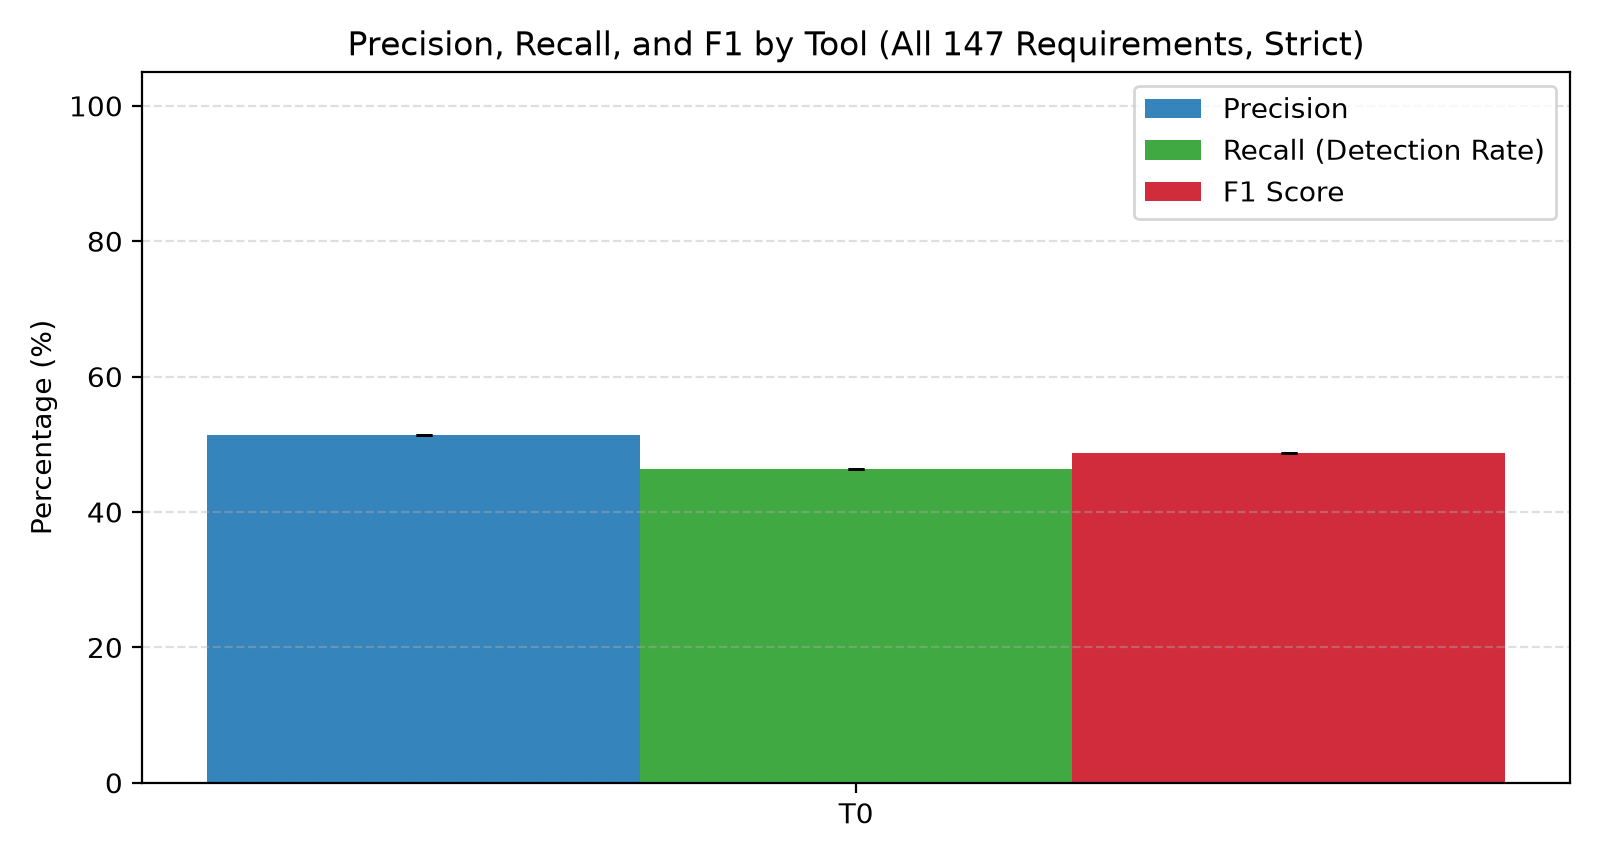
\includegraphics[width=0.9\textwidth]{prf1_by_tool.png}
\caption{Precision, Recall và $F_1$ trên PURE; đường nét đứt là $F_1$ khi gắn cờ mọi yêu cầu}
\label{fig:prf1}
\end{figure}

Khi không có kỹ năng, $F_1$ của LLM (T1: \numFTone\%, T3: \numFTthree\%) không cao hơn T0 (\numFTzero\%). Mọi công cụ đều vượt mốc tham chiếu ``gắn cờ mọi yêu cầu cho mọi loại'' ($F_1$ \numFFlagAll\%), nghĩa là các công cụ có chọn lọc thật. Về mặt thực tế, người rà soát phải đọc khoảng \numEffortTone{} cảnh báo của T1, hay \numEffortTfour{} cảnh báo của T4, để gặp một khiếm khuyết có trong nhãn chuẩn.

Từ kết quả thu được, có thể thấy rằng công cụ LLM có độ bao phủ rất cao nhưng độ chính xác thấp; nếu chỉ dùng câu lệnh thuần, LLM chưa vượt được một bộ dò dựa trên luật đơn giản.

\subsection{Tác động của kỹ năng (RQ2)}
Hình~\ref{fig:skill} so sánh $F_1$ khi dùng câu lệnh thuần và khi dùng kỹ năng. Kỹ năng tăng $F_1$ ở cả hai mô hình với mức gần như nhau: $+\numSkillDFHydro$ điểm phần trăm với Hydrogen (KTC 95\%: [\numSkillLoHydro; \numSkillHiHydro]) và $+\numSkillDFNeon$ điểm với Neon (KTC 95\%: [\numSkillLoNeon; \numSkillHiNeon]). Cả hai khoảng tin cậy đều không chứa 0. Cụ thể, Precision tăng lần lượt \numSkillDPHydro{} và \numSkillDPNeon{} điểm, trong khi Recall chỉ giảm \numSkillDRHydro{} và \numSkillDRNeon{} điểm: các quy tắc loại trừ trong kỹ năng giúp mô hình bỏ bớt cảnh báo yếu.

\begin{figure}[H]
\centering
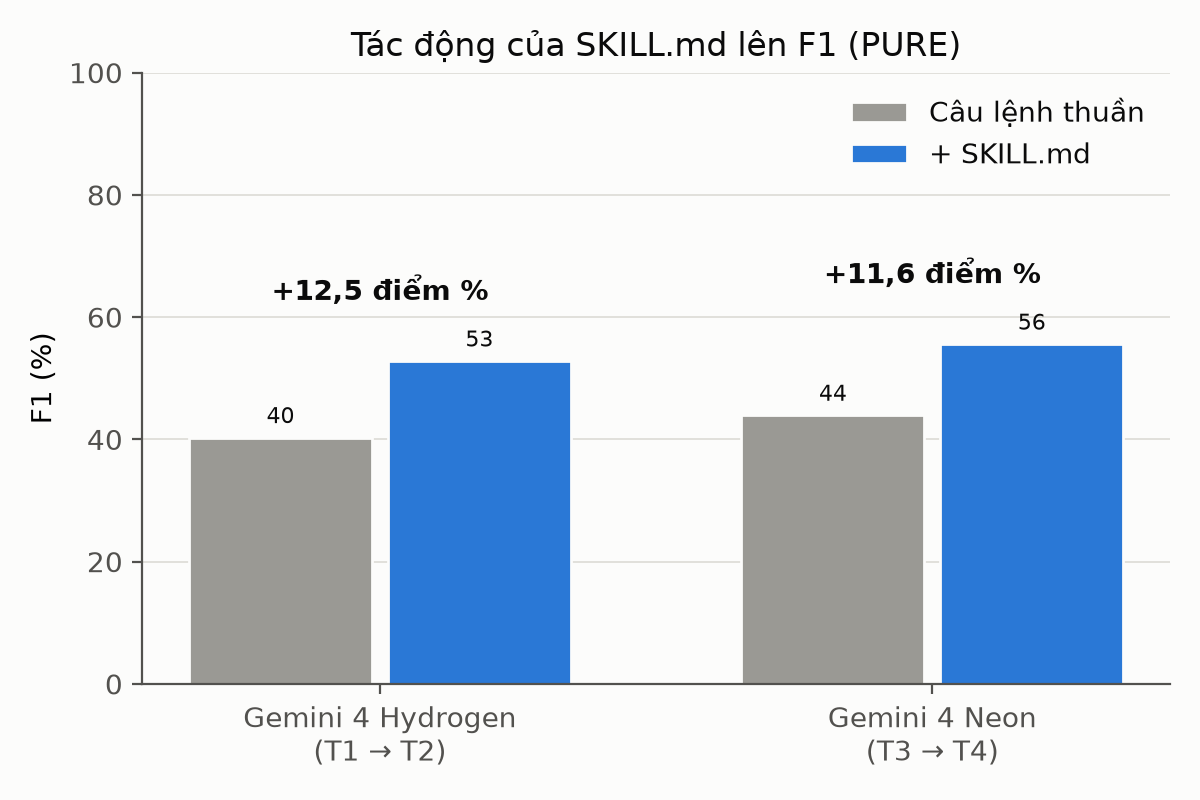
\includegraphics[width=0.62\textwidth]{skill_effect.png}
\caption{$F_1$ trên PURE với câu lệnh thuần và với kỹ năng}
\label{fig:skill}
\end{figure}

So sánh hai mô hình, Neon tốt hơn Hydrogen $+\numModelDFPlain$ điểm $F_1$ khi dùng câu lệnh thuần và $+\numModelDFSkill$ điểm khi có kỹ năng, nhưng chạy chậm gấp khoảng hai lần (\numDurTthree{} so với \numDurTone{} giây mỗi lượt). Như vậy, việc trang bị kỹ năng mang lại lợi ích lớn hơn khoảng 3--4 lần so với việc chọn mô hình.

\subsection{Kết quả theo loại khiếm khuyết (RQ3)}
Vì Recall của LLM đều từ 91\% trở lên ở mọi loại, khác biệt giữa các loại thể hiện chủ yếu ở Precision và $F_1$ (Bảng~\ref{tab:pure_by_type}, Hình~\ref{fig:by_type}). Mâu thuẫn là loại dễ nhất, $F_1$ của LLM đạt từ \numFConTthree\% đến \numFConTtwo\%, vì các yêu cầu trùng lặp trong tài liệu Peering được mọi công cụ phát hiện. Thiếu sót là loại khó nhất, $F_1$ chỉ từ \numFIncTone\% đến \numFIncTfour\% (T0: \numFIncTzero\%), do ranh giới giữa ``thiếu thông tin thật'' và ``có thể bổ sung thêm chi tiết'' mang tính phán đoán cao. Với lỗi mơ hồ, kỹ năng giúp nhiều nhất (T1 \numFAmbTone\% lên T2 \numFAmbTtwo\%), và đáng chú ý là T0 cũng đạt \numFAmbTzero\%, vì lỗi mơ hồ thường gắn với từ khóa như ``\textit{easy}'' hay ``\textit{fast}''.

\begin{table}[H]
\centering
\caption{Precision (P), Recall (R) và $F_1$ theo loại khiếm khuyết trên PURE}
\label{tab:pure_by_type}
\small
\begin{tabular}{lccccccccc}
\toprule
& \multicolumn{3}{c}{\textbf{Ambiguity}} & \multicolumn{3}{c}{\textbf{Incompleteness}} & \multicolumn{3}{c}{\textbf{Inconsistency}} \\
\textbf{Công cụ} & P & R & $F_1$ & P & R & $F_1$ & P & R & $F_1$ \\
\midrule
T0 & 0{,}92 & 0{,}52 & 0{,}67 & 0{,}18 & 0{,}32 & 0{,}23 & 1{,}00 & 0{,}44 & 0{,}62 \\
T1 & 0{,}22 & 1{,}00 & 0{,}37 & 0{,}22 & 1{,}00 & 0{,}37 & 0{,}66 & 1{,}00 & 0{,}79 \\
T2 & 0{,}43 & 0{,}94 & 0{,}59 & 0{,}27 & 0{,}94 & 0{,}41 & 0{,}80 & 1{,}00 & 0{,}89 \\
T3 & 0{,}27 & 1{,}00 & 0{,}42 & 0{,}25 & 0{,}98 & 0{,}39 & 0{,}53 & 1{,}00 & 0{,}69 \\
T4 & 0{,}47 & 0{,}92 & 0{,}62 & 0{,}30 & 0{,}91 & 0{,}46 & 0{,}61 & 1{,}00 & 0{,}76 \\
\bottomrule
\end{tabular}

\end{table}

\begin{figure}[H]
\centering
\begin{subfigure}{0.49\textwidth}
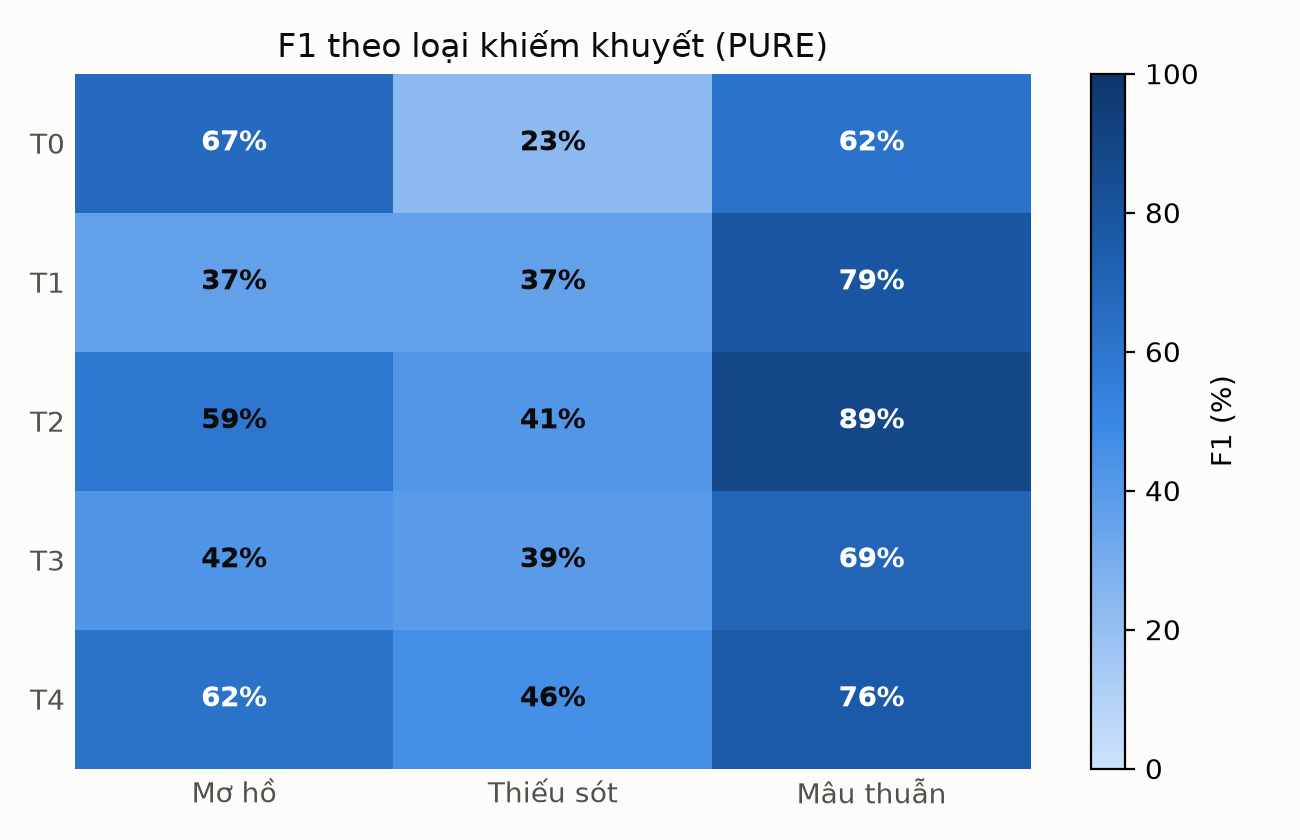
\includegraphics[width=\textwidth]{f1_heatmap.png}
\caption{$F_1$ theo loại}
\end{subfigure}
\begin{subfigure}{0.49\textwidth}
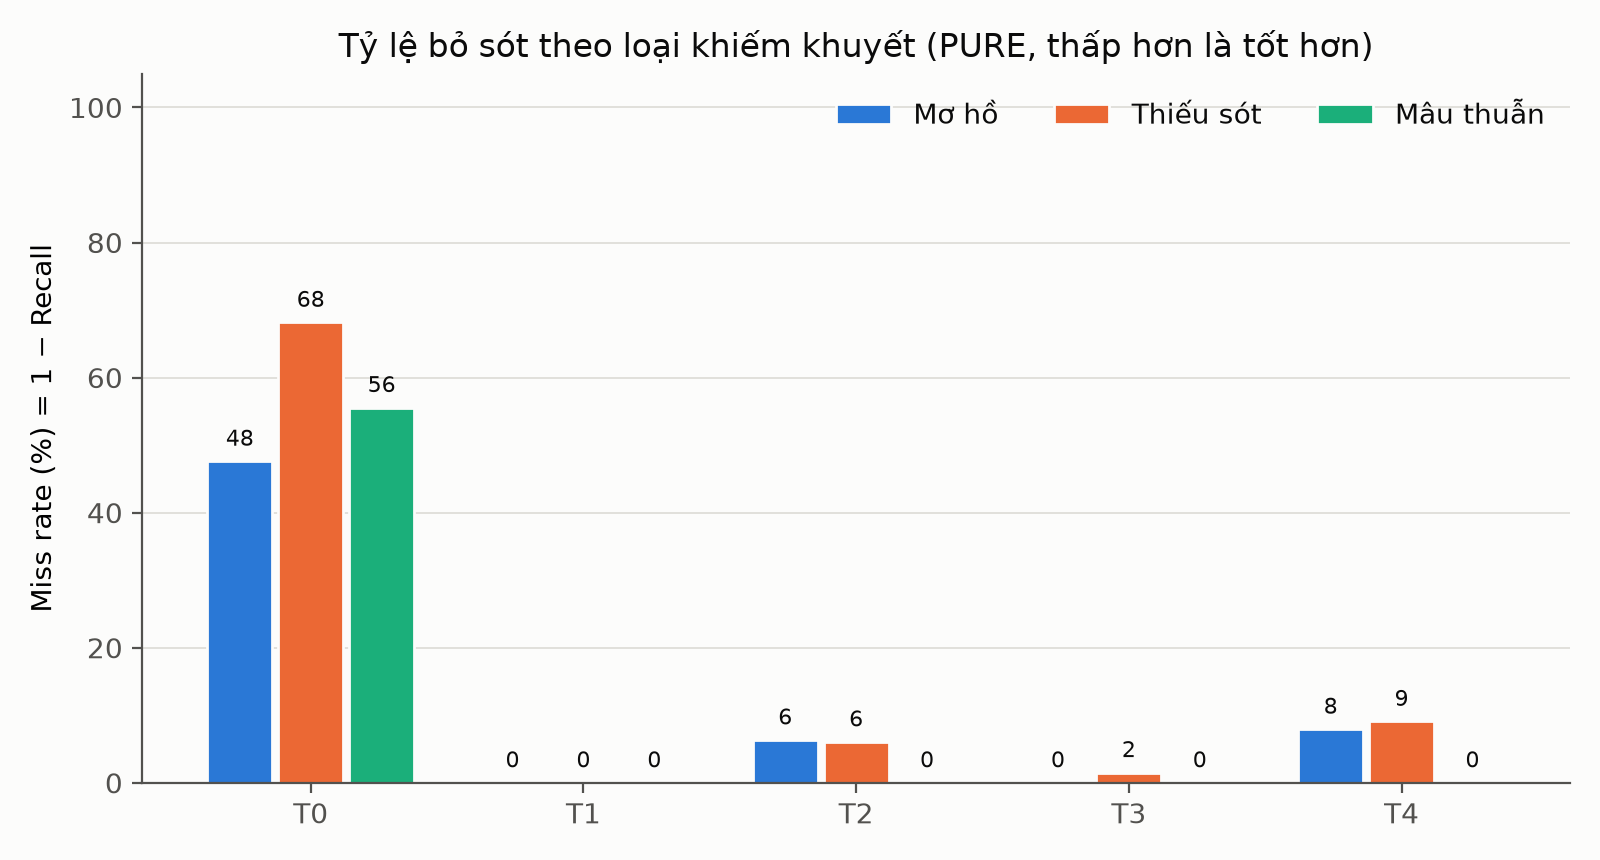
\includegraphics[width=\textwidth]{miss_rate_by_type.png}
\caption{Tỷ lệ bỏ sót theo loại}
\end{subfigure}
\caption{Kết quả theo loại khiếm khuyết trên PURE}
\label{fig:by_type}
\end{figure}

\subsection{Độ ổn định và chi phí (RQ4)}
Kết quả ổn định cao giữa 3 lượt chạy (Hình~\ref{fig:stability}): chỉ số Jaccard đạt từ \numJacTtwo{} đến \numJacTone{} và Fleiss' $\kappa$ từ \numFleissTthree{} đến \numFleissTone. Độ lệch chuẩn của $F_1$ giữa các lượt không quá \numFsdTthree{} điểm, nhỏ hơn nhiều so với tác động của kỹ năng, nên các kết luận ở RQ1--RQ3 không phụ thuộc vào một lượt chạy riêng lẻ. Toàn bộ 48 lượt chạy mất \numAgyMinutes{} phút và \numAgyMTokens{} triệu token; mỗi lượt Hydrogen mất khoảng \numDurTone--\numDurTtwo{} giây, mỗi lượt Neon khoảng \numDurTfour--\numDurTthree{} giây.

\begin{figure}[H]
\centering
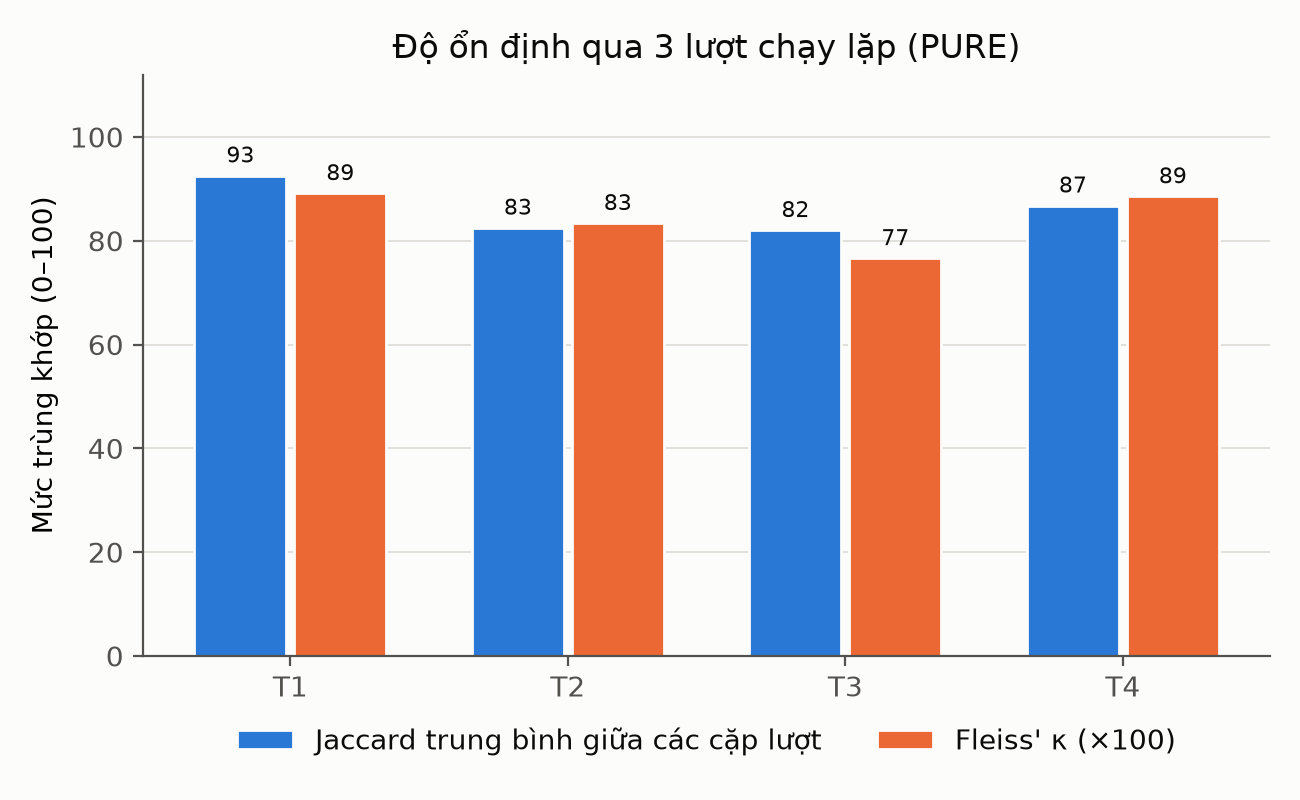
\includegraphics[width=0.62\textwidth]{stability.png}
\caption{Độ ổn định qua 3 lượt chạy trên PURE}
\label{fig:stability}
\end{figure}

\subsection{Tài liệu cấy lỗi}
\label{sec:seeded_sanity}
Trên tài liệu cấy lỗi, mọi công cụ LLM đạt $F_1$ từ \numFSeedTone\% đến \numFSeedTfour\% (T0: \numFSeedTzero\%). Các lỗi được cấy theo mẫu điển hình nên quá dễ với LLM; tài liệu này chỉ xác nhận công cụ phát hiện được khiếm khuyết điển hình, không dùng để so sánh các công cụ. Hai phân tích độ nhạy cho thấy kết luận không đổi: coi một khiếm khuyết vô tình có trong yêu cầu ``sạch'' là lỗi thật làm $F_1$ thay đổi tối đa \numSDMaxShift{} điểm, và việc lộ số lượng lỗi trước khi sửa (mục~\ref{sec:leak}) chỉ làm $F_1$ tăng tối đa \numLeakMaxShift{} điểm.

\section{Phân tích lỗi}
\label{sec:error_analysis}
Precision thấp đặt ra câu hỏi: các cảnh báo ``thừa'' là nhiễu, hay là khiếm khuyết thật mà nhãn chuẩn bỏ qua? Nhóm lấy mẫu 30 trường hợp bất đồng trên PURE, gồm toàn bộ 5 nhãn chuẩn mà có lượt chạy bỏ sót và 25 trong 172 cảnh báo chỉ do công cụ đưa ra. Các trường hợp được trộn và ẩn nguồn trước khi đánh giá.

Một tác tử Claude Opus mới, không biết nguồn, đánh giá rằng trong \numAIRevN{} cảnh báo chỉ do công cụ đưa ra có \numAIRevReal{} khiếm khuyết thật, \numAIRevBorder{} trường hợp ở ranh giới và \numAIRevNot{} không phải khiếm khuyết. Như vậy khoảng \numAIRevRealLo--\numAIRevRealHi\% cảnh báo ``thừa'' có thể là lỗi thật, nên Precision thật của công cụ có lẽ cao hơn con số ở Bảng~\ref{tab:overall_pure}. Ngược lại, \numAIRevExpReal/\numAIRevExpN{} nhãn chuẩn bị bỏ sót được xác nhận là lỗi thật. Nguyên nhân chính của cảnh báo sai là \textbf{đòi hỏi quá mức} (\numAIRevOverLiteral{} trường hợp: yêu cầu đã rõ và kiểm chứng được nhưng công cụ vẫn đòi bổ sung) và \textbf{gắn cờ văn bản không phải yêu cầu} (\numAIRevNonReq{} trường hợp: ghi chú hoặc câu giải thích lẫn vào yêu cầu khi trích xuất PURE). Một số ví dụ tiêu biểu:
\begin{itemize}
  \item \textbf{Lỗi thật mà nhãn chuẩn bỏ qua} (PE-004, cả 12 lượt chạy đều gắn cờ): ``\textit{Resource provisioning, delegation and reservation policies are in place}''. Yêu cầu không nêu chính sách nào nên không thể kiểm chứng.
  \item \textbf{Lỗi thật mà công cụ bỏ sót} (PE-007): ``\textit{Malicious requests are detected and rejected}''. Không có tiêu chí xác định thế nào là yêu cầu độc hại.
  \item \textbf{Đòi hỏi quá mức} (GJ-013): ``\textit{The system shall be able to retrieve 200 products per second}'' bị coi là cụm từ yếu, dù con số đã làm yêu cầu kiểm chứng được.
  \item \textbf{Không phải yêu cầu} (GJ-005): cụm ``\textit{easy of use}'' bị coi là mơ hồ, nhưng nó nằm trong câu giải thích, không phải trong yêu cầu ``\textit{Must use a SQL based database}''.
\end{itemize}

\ifhumancheck
Lượt rà soát độc lập thay người (mục~\ref{sec:human_check}) cũng đánh giá 30 trường hợp này mà không biết nguồn và xác nhận \numHCRealRate\% cảnh báo chỉ do công cụ đưa ra là khiếm khuyết thật, nằm trong khoảng ước lượng ở trên. Tính theo tỷ lệ này cho từng loại, Precision điều chỉnh trên PURE là \numPAdjTone\% (T1), \numPAdjTtwo\% (T2), \numPAdjTthree\% (T3), \numPAdjTfour\% (T4) và \numPAdjTzero\% (T0).
\else
\textbf{[Đang chờ kết quả rà soát độc lập: tỷ lệ cảnh báo thừa được xác nhận là lỗi thật và Precision điều chỉnh.]}
\fi

\section{Hạn chế}
\label{sec:threats}
Kết quả của báo cáo cần được hiểu trong các giới hạn sau:
\begin{itemize}
  \item \textbf{Nhãn chuẩn do AI tạo.} Nhãn chuẩn không do kỹ sư yêu cầu chuyên nghiệp gắn. Nhóm giảm thiểu rủi ro bằng hai lượt độc lập, đo $\kappa$, kiểm định trên tài liệu cấy lỗi, người rà soát thứ hai và một lượt rà soát độc lập thay người. Cả hai lượt rà soát này đều do Claude thực hiện, nên nhãn chuẩn \textbf{chưa được con người kiểm tra}; mức đồng thuận về thiếu sót còn thấp. Phân tích lỗi cho thấy nhãn chuẩn khá khắt khe, nên Precision báo cáo là cận dưới.
  \item \textbf{Chỉ hai mô hình của cùng một nhà cung cấp.} Hai mô hình Gemini trùng khoảng 80\% phát hiện, nên kết luận chỉ chắc chắn cho họ mô hình này, dù tác động của kỹ năng lặp lại ở cả hai.
  \item \textbf{Kỹ năng và nhãn chuẩn dùng chung bảng phân loại.} Một phần lợi ích của kỹ năng có thể đến từ việc khớp quy ước gắn nhãn. Các ví dụ trong kỹ năng đã được thay bằng ví dụ ngoài bộ dữ liệu.
  \item \textbf{Quy mô nhỏ và khả năng lộ dữ liệu huấn luyện.} Chỉ có 107 yêu cầu thật; bộ PURE công khai từ năm 2017 nên có thể đã nằm trong dữ liệu huấn luyện của LLM. Tài liệu cấy lỗi mới viết giúp kiểm soát phần nào rủi ro này.
  \item \textbf{Phiên bản mô hình thay đổi.} Bí danh mô hình không cố định phiên bản; nhóm ghi lại phiên bản công cụ, ngày chạy và chạy lặp 3 lần.
\end{itemize}

% ============================================================
%  CHƯƠNG 5: KẾT LUẬN
% ============================================================
\chapter{Kết luận}

\section{Kết quả đạt được}
Với đề tài A1, báo cáo đã đánh giá bốn cấu hình công cụ AI dựa trên hai mô hình Gemini 4, cùng một bộ dò dựa trên luật, trên 107 yêu cầu thật của bộ PURE, đối chiếu với nhãn chuẩn được đóng băng trước khi chạy công cụ. Cụ thể, các kết quả chính gồm:
\begin{itemize}
  \item \textbf{RQ1:} công cụ LLM có tỷ lệ phát hiện đúng rất cao (Recall từ \numRTfour\% đến \numRTone\%, tỷ lệ bỏ sót không quá \numMissTfour\%) nhưng Precision thấp (\numPTone--\numPTfour\%); $F_1$ tốt nhất là \numFTfour\% (T4).
  \item \textbf{RQ2:} tệp kỹ năng tăng $F_1$ khoảng 12 điểm phần trăm ở cả hai mô hình, với ý nghĩa thống kê, chủ yếu nhờ tăng Precision.
  \item \textbf{RQ3:} thiếu sót là loại khó nhất, mâu thuẫn là loại dễ nhất; với lỗi mơ hồ, bộ dò dựa trên luật đã cạnh tranh được với LLM.
  \item \textbf{RQ4:} kết quả ổn định qua các lượt chạy (Jaccard từ \numJacTtwo{} đến \numJacTone).
\end{itemize}
Phân tích lỗi cho thấy một phần đáng kể cảnh báo ``thừa'' là khiếm khuyết thật. Vì vậy, công cụ AI có kỹ năng phù hợp nhất với vai trò trợ lý sàng lọc: công cụ đề xuất, con người quyết định. Bộ dò dựa trên luật có thể được dùng trước như một bước lọc nhanh, nhất là với lỗi mơ hồ.

\section{Hướng phát triển}
Mặc dù kết quả đạt được là tích cực, nghiên cứu có thể được mở rộng theo các hướng sau:
\begin{itemize}
  \item Xây dựng nhãn chuẩn đầy đủ do kỹ sư yêu cầu gắn nhãn, và mở rộng sang tài liệu SRS tiếng Việt thực tế.
  \item Đánh giá thêm mô hình của các nhà cung cấp khác để kiểm chứng tính tổng quát của tác động kỹ năng.
  \item Kết hợp bộ dò dựa trên luật với tác tử LLM có kỹ năng, và đo lợi ích trên thời gian rà soát thực tế của người dùng.
\end{itemize}

% ============================================================
%  TÀI LIỆU THAM KHẢO
% ============================================================
\chapter*{Tài liệu tham khảo}
\addcontentsline{toc}{chapter}{Tài liệu tham khảo}

\begin{enumerate}[leftmargin=2.2em,label={[\arabic*]}]
  \bibitem{ieee830}
  IEEE Computer Society. (1998). \textit{IEEE Std 830-1998: IEEE Recommended Practice for Software Requirements Specifications}. IEEE.

  \bibitem{iso29148}
  ISO/IEC/IEEE. (2018). \textit{ISO/IEC/IEEE 29148:2018: Systems and software engineering --- Life cycle processes --- Requirements engineering}. International Organization for Standardization.

  \bibitem{berry2003}
  Berry, D. M., Kamsties, E., \& Krieger, M. M. (2003). \textit{From Contract Drafting to Software Specification: Linguistic Sources of Ambiguity} (A Handbook, Version 1.0). University of Waterloo. \url{https://cs.uwaterloo.ca/~dberry/handbook/ambiguityHandbook.pdf}

  \bibitem{ferrari2017}
  Ferrari, A., Spagnolo, G. O., \& Gnesi, S. (2017). PURE: A Dataset of Public Requirements Documents. \textit{Proceedings of the 25th IEEE International Requirements Engineering Conference (RE)}, pp. 502--505. DOI: 10.1109/RE.2017.29.

  \bibitem{femmer2017}
  Femmer, H., Méndez Fernández, D., Wagner, S., \& Eder, S. (2017). Rapid quality assurance with Requirements Smells. \textit{Journal of Systems and Software}, 123, 190--213. DOI: 10.1016/j.jss.2016.02.047.

  \bibitem{fabbrini2001}
  Fabbrini, F., Fusani, M., Gnesi, S., \& Lami, G. (2001). The Linguistic Approach to the Natural Language Requirements Quality: Benefit of the use of an Automatic Tool. \textit{Proceedings of the 26th Annual NASA Goddard Software Engineering Workshop}, Greenbelt, MD, USA.

  \bibitem{fabbrini2005}
  Fabbrini, F., Fusani, M., Gnesi, S., Lami, G., \& Trentanni, G. (2005). An Automatic Tool for the Analysis of Natural Language Requirements. \textit{Computer Systems Science and Engineering}.

  \bibitem{zhao2021}
  Zhao, L., Alhoshan, W., Ferrari, A., Letsholo, K. J., Ajagbe, M. A., Chioasca, E.-V., \& Batista-Navarro, R. T. (2021). Natural Language Processing (NLP) for Requirements Engineering (RE): A Systematic Mapping Study. \textit{ACM Computing Surveys}, 54(3).

  \bibitem{lubos2024}
  Lubos, S., Felfernig, A., Tran, T. N. T., Garber, D., El Mansi, M., Erdeniz, S. P., \& Le, V.-M. (2024). Leveraging LLMs for the Quality Assurance of Software Requirements. \textit{Proceedings of the 32nd IEEE International Requirements Engineering Conference (RE)}, pp. 389--397.

  \bibitem{ronanki2025}
  Ronanki, K., Arvidsson, S., \& Axell, J. (2025). Prompt Engineering Guidelines for Using Large Language Models in Requirements Engineering. \textit{51st Euromicro Conference on Software Engineering and Advanced Applications (SEAA)}, Lecture Notes in Computer Science. DOI: 10.1007/978-3-032-04207-1\_17.
\end{enumerate}

% ============================================================
%  PHỤ LỤC
% ============================================================
\appendix
\chapter{Phụ lục}

\section{Tệp kỹ năng}
\label{app:skill}
\lstinputlisting[caption={Tệp kỹ năng được nạp cho T2 và T4}]{../prompt/SKILL.md}

\section{Câu lệnh}
Hai câu lệnh dưới đây giống hệt nhau, trừ dòng đầu của câu lệnh kèm kỹ năng.
\lstinputlisting[caption={Câu lệnh thuần (T1, T3)}]{../prompt/plain.txt}
\lstinputlisting[caption={Câu lệnh kèm kỹ năng (T2, T4)}]{../prompt/skill.txt}

\section{Mã nguồn và khả năng tái lập}
\label{app:repro}
Toàn bộ dữ liệu, nhãn chuẩn (kèm mã băm), kết quả 48 lượt chạy, mã nguồn chấm điểm và tệp nguồn của báo cáo được công bố tại \url{https://github.com/feiluvnana/REPORT-SEMINAR-1}. Tệp \texttt{README.md} hướng dẫn tái lập từng bước; mọi con số trong báo cáo được sinh tự động từ kết quả, nên chạy lại chương trình sẽ cho đúng các bảng và hình ở Chương 4.

\end{document}
